\documentclass[../main.tex]{subfiles}

\makeatletter
\@ifundefined{fromRoot}{%
  \newcommand{\fromRoot}[1]{../#1}
  
  \usepackage{xr}
  \externaldocument{../main}
}{}

\def\input@path{{\subfix{../}}}
%or: \def\input@path{{/path/to/folder/}{/path/to/other/folder/}}
\makeatother

\graphicspath{
  {\subfix{../}}
  {\subfix{./figures}}
  {\subfix{../figures}}
  {\subfix{./figures/logos-thesis/}}
  {\subfix{../figures/logos-thesis/}}
  {\subfix{./figures/rtexps-pics/}}
  {\subfix{../figures/rtexps-pics/}}
}

\hypersetup{
    pdfauthor   = {Camille MONIÈRE},
    pdftitle    = {Th\`{e}se (Présentation: étude algorithmique)},
    pdfsubject  = {Th\`{e}se (Présentation: étude algorithmique)},
%    pdfkeywords = {mots-cl\'{e}s},
}

\begin{document}

\section{Étude algorithmique}

\subsection{Sensibilité à un facteur d'échelle}

\begin{frame}{\subsecname}
  \begin{columns}
    \begin{column}{.5\linewidth}
      \centering
      \begin{itemize}
        \item L'utilisation de dispositif bas-coûts implique une instabilité du gain des amplificateurs.
        \item Constat d'une forte perte de performance de détection.
      \end{itemize} \vspace*{1 em}

      \includegraphics[width=.75\linewidth]{figures/pgfplots/gain_gained.pdf}
      \captionof{figure}{Gain en dB variable}
    \end{column}
    \begin{column}{.5\linewidth}
      \includegraphics[width=\linewidth]{figures/pgfplots/score_function_gained.pdf}
    \end{column}
  \end{columns}
\end{frame}

\begin{frame}{Solution : normalisation}
  \begin{columns}
    \begin{column}{.5\linewidth}
      \centering
      Normalisation des maximums de corrélation avant accumulation par la norme-2 : $$\mnorm{2}(\vect{y}_n) = \sqrt{\sum_{i = 0}^{q - 1} y_n(i)}$$\\
      Impact léger sur les performances de détection\footnotemark.
      
      \vspace*{1 em}

      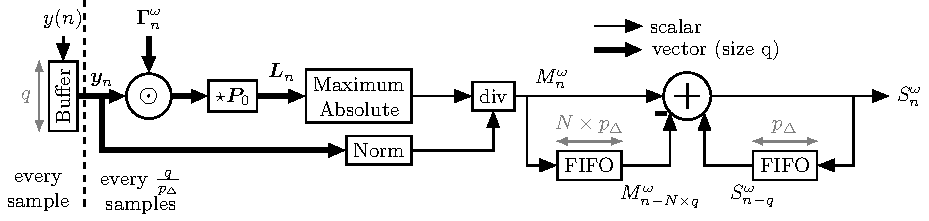
\includegraphics[width=\linewidth]{figures/tikzpicture/score_proc_unit_stdl.pdf}
    \end{column}
    \begin{column}{.5\linewidth}
      \includegraphics[width=\linewidth]{figures/pgfplots/score_function_normed.pdf}
    \end{column}
  \end{columns}
  \footnotetext{Une étude approfondie est disponible dans le manuscrit.}
\end{frame}



\subsection{Corrélation glissante dans le temps (\emph{Time sliding})}

\begin{frame}{Criticité de la tache de corrélation}
  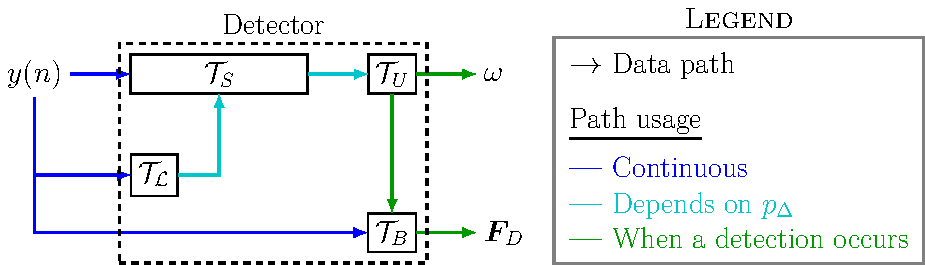
\includegraphics[width=\linewidth]{figures/tikzpicture/tasks_dep_stdl.pdf}
  \begin{center}
    \textcolor{RoyalBlue}{TODO}
  \end{center}
\end{frame}

\begin{frame}{Méthode par FFT}
  \centering
  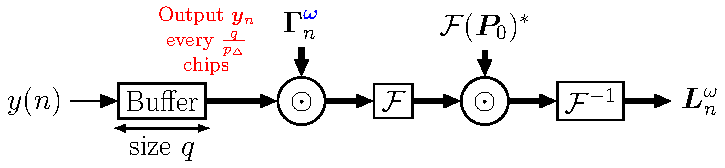
\includegraphics[width=.6\linewidth, height=.7\textheight, keepaspectratio=true]{figures/tikzpicture/arch_fft_sync_stdl.pdf}
  \begin{center}
    \textcolor{RoyalBlue}{TODO}
  \end{center}
\end{frame}

\begin{frame}{Méthode par TS : \textit{data shift}}
  \centering
  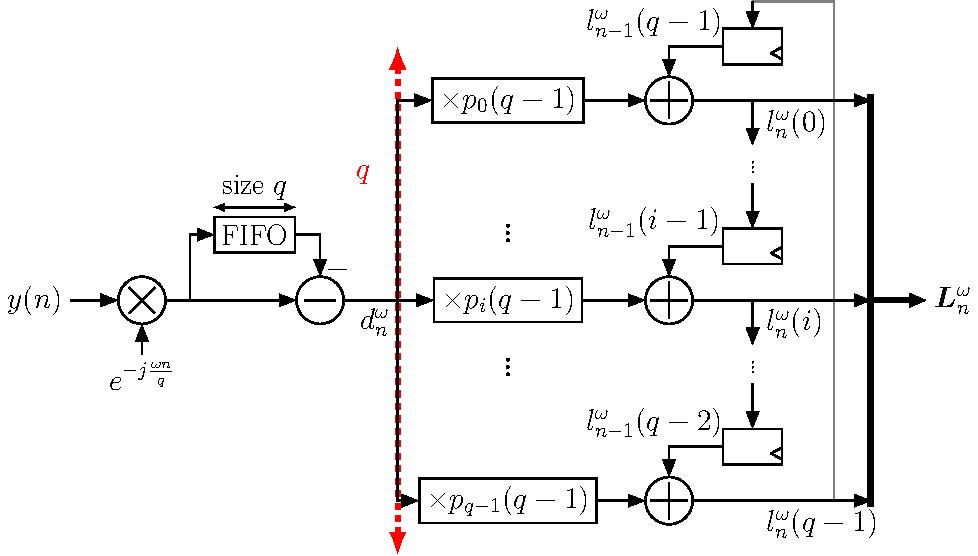
\includegraphics[width=\linewidth, height=.7\textheight, keepaspectratio=true]{figures/tikzpicture/arch_statts_sync_stdl.pdf}
  \begin{center}
    \textcolor{RoyalBlue}{TODO}
  \end{center}
\end{frame}

\begin{frame}{Méthode par TS : \textit{index shift}}
  \centering
  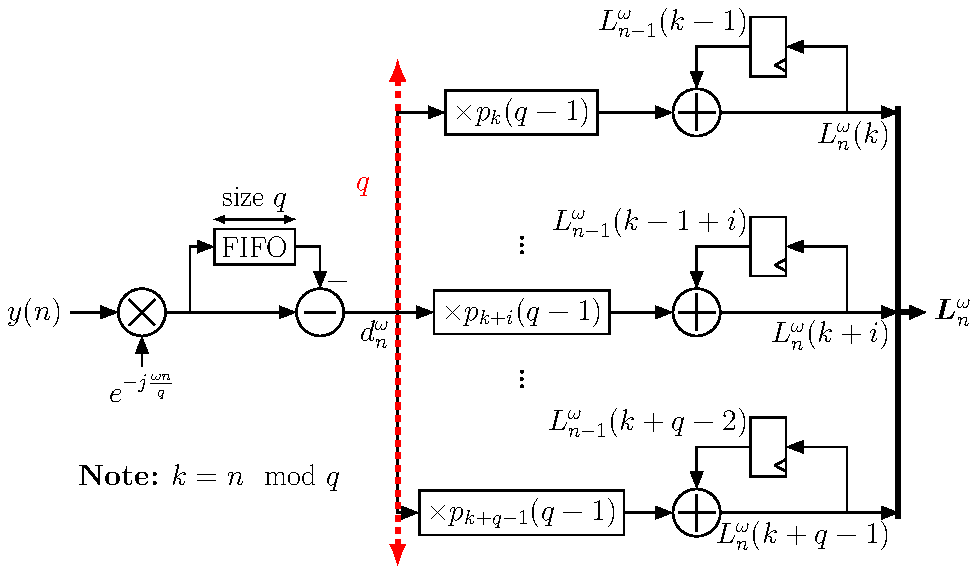
\includegraphics[width=\linewidth, height=.71\textheight, keepaspectratio=true]{figures/tikzpicture/arch_subts_sync_stdl.pdf}
  \begin{center}
    \textcolor{RoyalBlue}{TODO}
  \end{center}
\end{frame}

\end{document}
